%!TEX root = ../problems.tex
\begin{task}
	Найти спектр прямоугольного сигнала $S(t)=A\qty(-\H(t)+\H(t-t_1))$.
	Нарисовать график $\abs{S(\omega)}$.
\end{task}

\begin{proof}[\rm{\textbf{Решение}}]
	Продифференцируем $S(t)$:
	\begin{equation}
		\dv{S}{t}=A(-\delta(t)+\delta(t-t_1))
	\end{equation}
	По свойству дифференцирования преобразования Фурье:
	\begin{equation}
		S'(\omega)=i \omega S(\omega) 
			\quad\Longrightarrow\quad
			S(\omega)=\frac{S'(\omega)}{i \omega}
	\end{equation}
	\begin{gather*}
		S'(\omega)=A\newint (\delta(t-t_1)-\delta(t))e^{-i \omega t} \dd{t}
			=A(-1 +e^{-i \omega t}) = A(e^{-i \omega t} -1)
	\end{gather*}
	Получаем:
	\begin{equation}
		S(\omega)=\frac{A}{i \omega} (e^{-i \omega t_1}-1)
	\end{equation}
	Вынесем за скобки $e^{-\frac{i \omega t_1}{2}}$:
	\begin{equation}
		-\frac{A}{i \omega} e^{-\frac{i \omega t_1}{2}}
		%
		\underbrace{
			(e^{\frac{i \omega t_1}{2}} 
			-e^{-\frac{i \omega t_1}{2}})}
		%
			_{\displaystyle 2i\sin(\frac{\omega t_1}{2})}=
		%
		\frac{-2A}{\omega}
			e^{-\frac{i \omega t_1}{2}}
			\cdot\sin(\frac{\omega t_1}{2})=\\
		%
		At_1e^{-i\qty(\frac{i \omega t_1}{2}-\pi)}\cdot 
		\frac{\sin(\frac{\omega t_1}{2})}{\qty(\omega t_1/2)}
	\end{equation}
	И окончательный ответ:
	\begin{equation}
		\abs{S(\omega)}=At_1
			\abs{
				\frac{\sin(\frac{\omega t_1}{2})}{\qty(\omega t_1/2)}
			},
	\end{equation}
	где $t_1$ -- длительность прямоугольного импульса.
	\begin{figure}[h!]
		\centering
		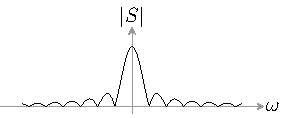
\includegraphics[scale=1.8]{ris/task5_out}		
		\caption{Спектр прямоугольного импульса}
		% \label{fig:figure1}
	\end{figure}

\end{proof} 